\subsection{An R and \protect\pbdR View of Parallel Hardware and Software}
\makesubcontentsslidessec

\begin{frame}{R Interfaces to Low-Level Native Tools}
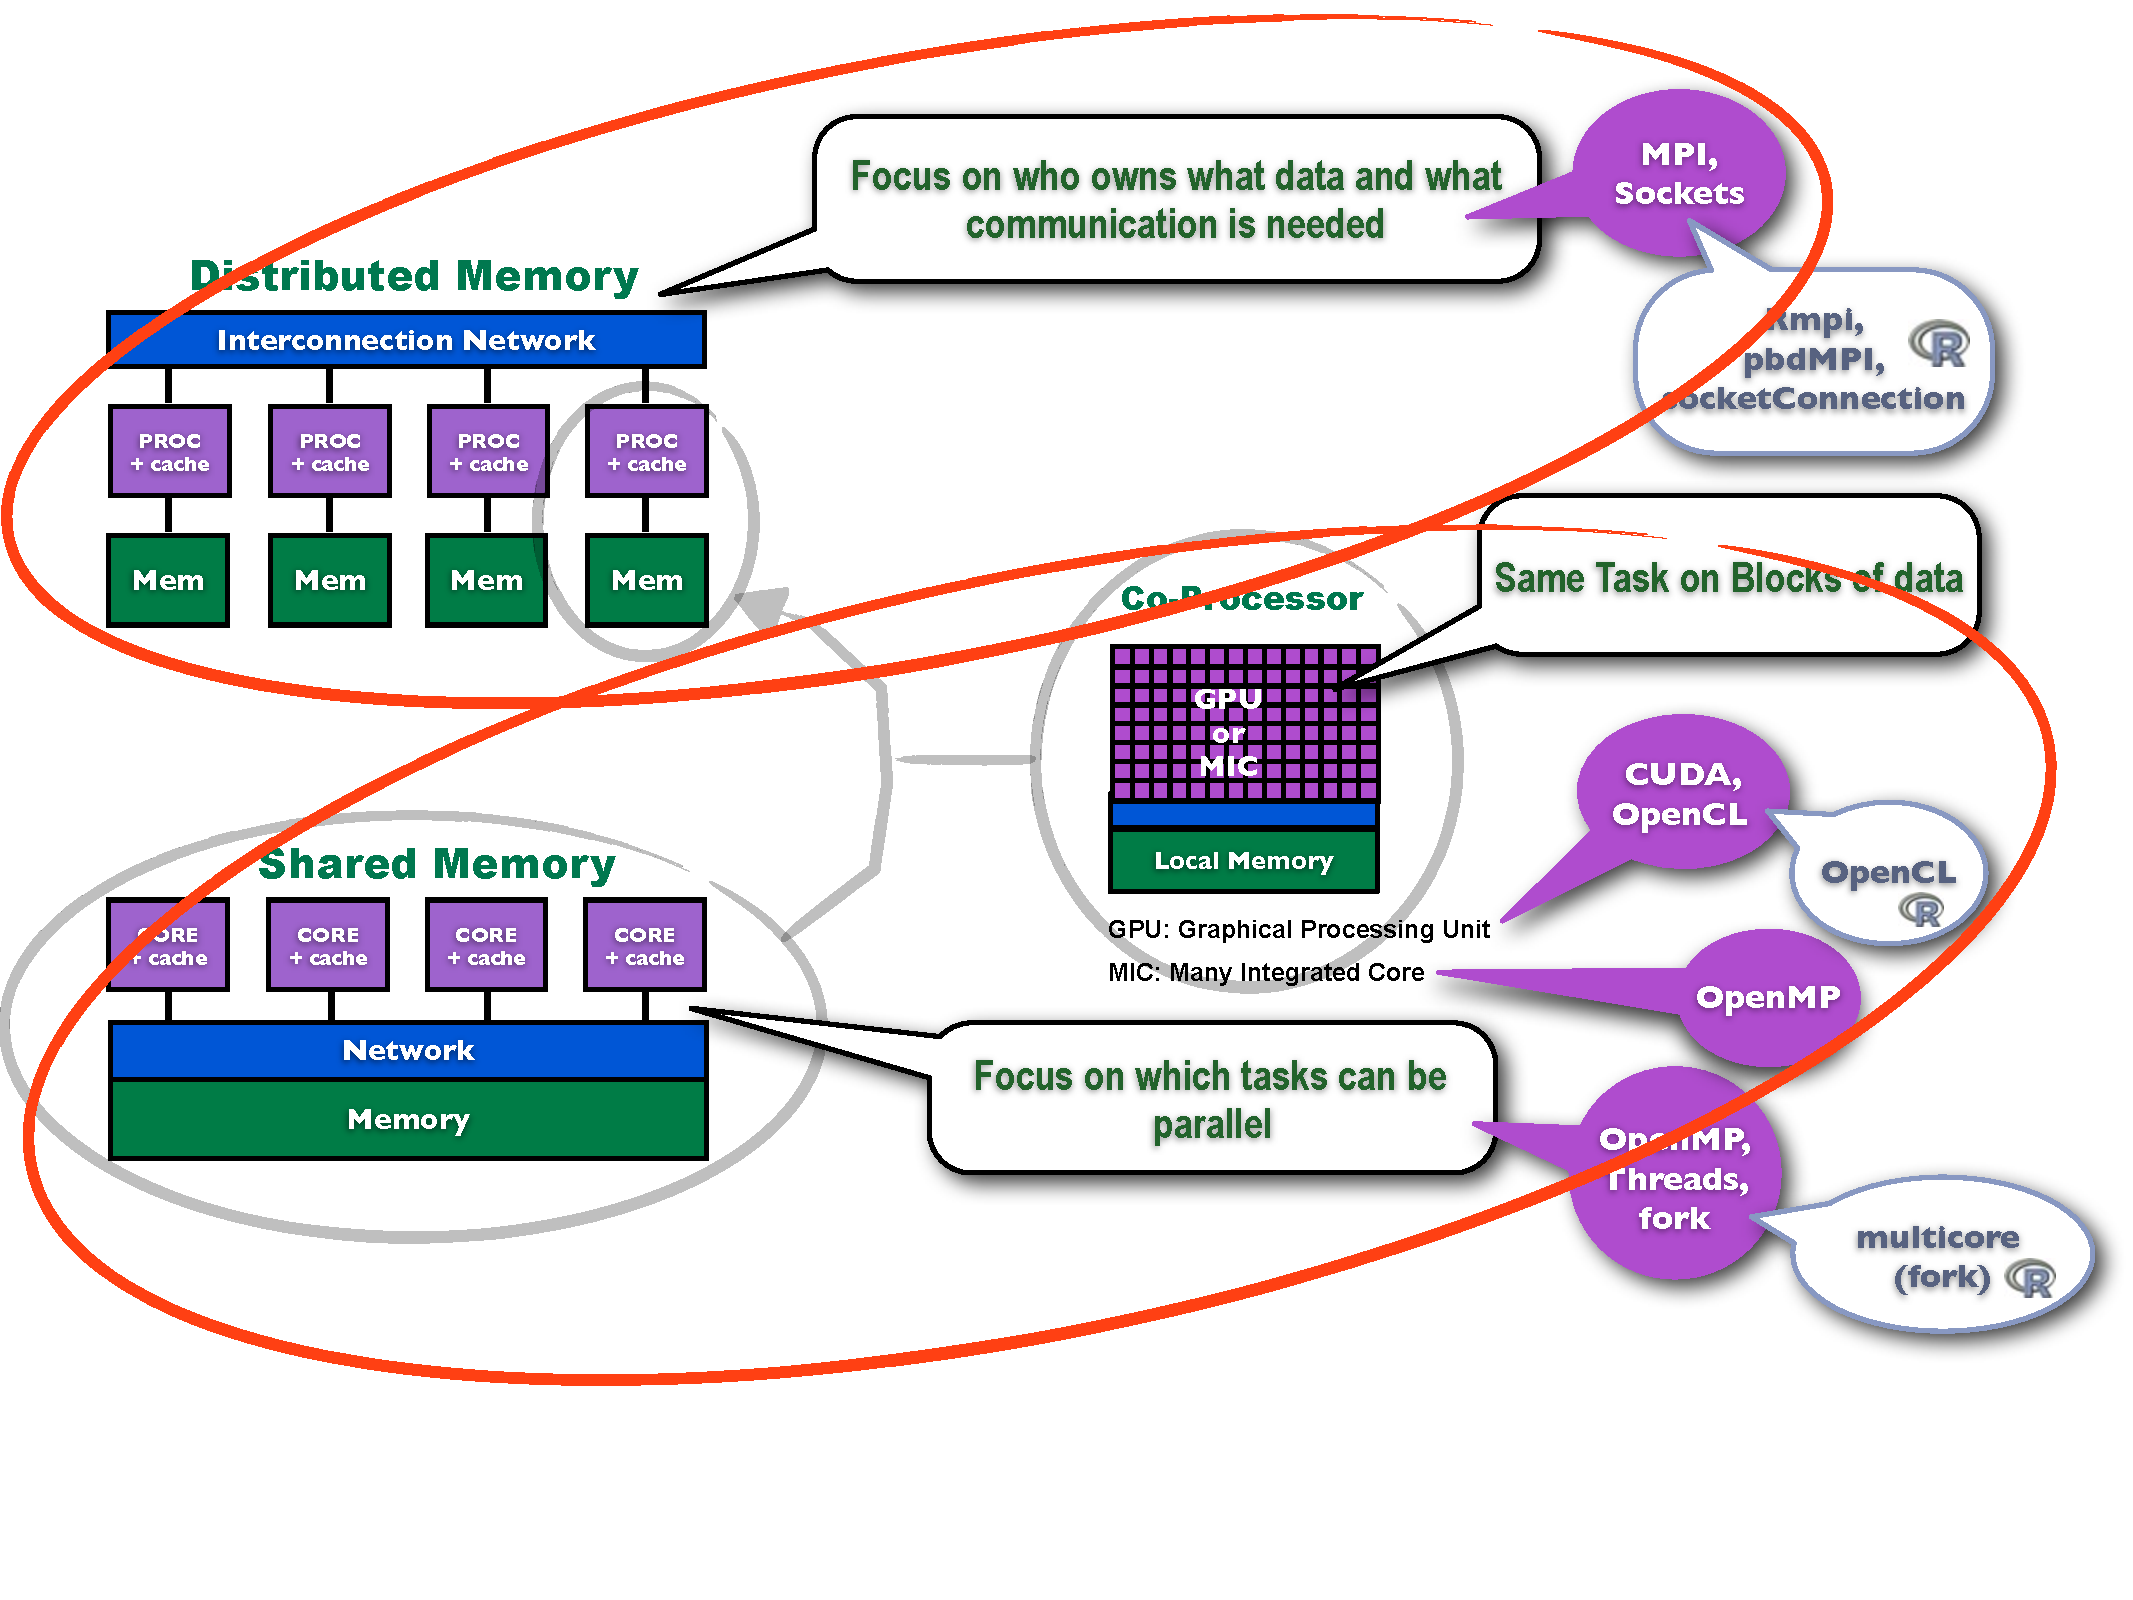
\includegraphics[height=\textheight]
{../common/pics/hardware/ParallelHardware10.pdf}
\end{frame}

\begin{frame}{Parallel Computing before Multicore}
\begin{minipage}{8.0cm}
  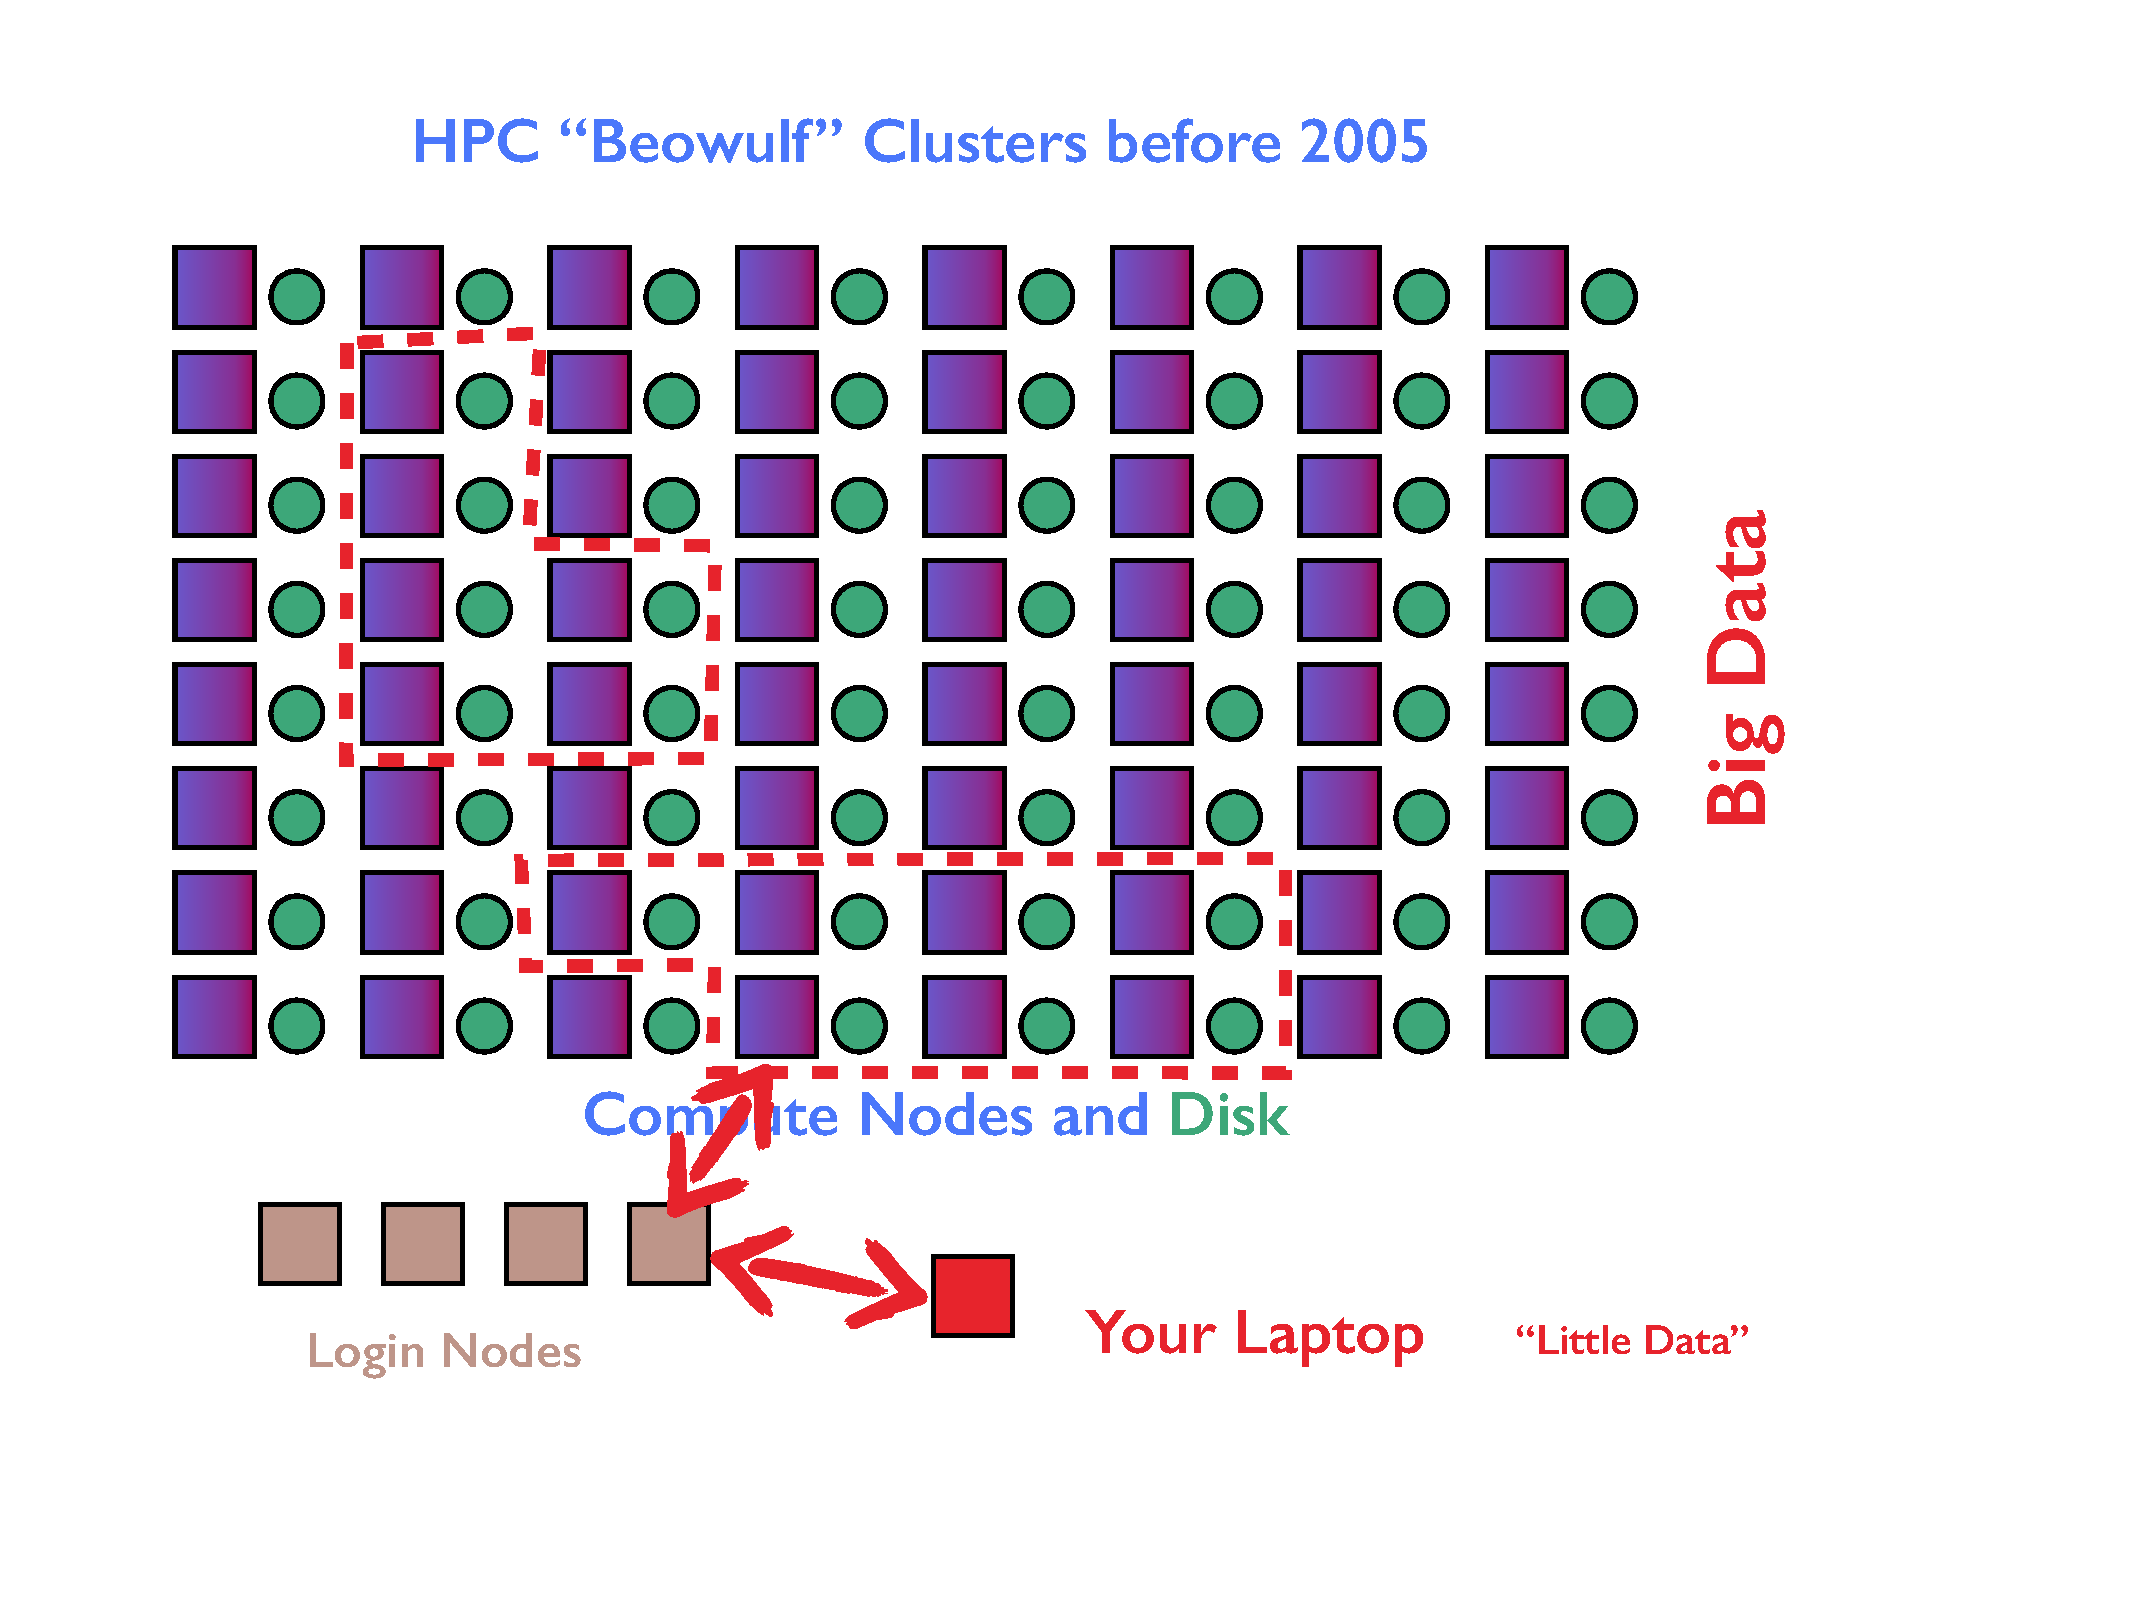
\includegraphics[trim=3cm 0cm 0cm 0cm,clip=true,height=0.9\textheight]
  {../common/pics/hardware/ParallelHardware22.pdf}\hfill
\end{minipage}
\hspace{1ex}
\begin{minipage}{3.6cm}\small
  \begin{block}{Software:}\pause
    \scriptsize MPI is mature, Map-Reduce emerges \\[1ex]
    Parallel Libraries: PBLAS, ScaLAPACK, PETSc, etc. \\[1ex]
    Resource Manager: PBS mature, HADOOP emerges
  \end{block}
\end{minipage}
\end{frame}

\begin{frame}{Multicore Emerges and Clusters become Diskless}
\begin{minipage}{8.0cm}
  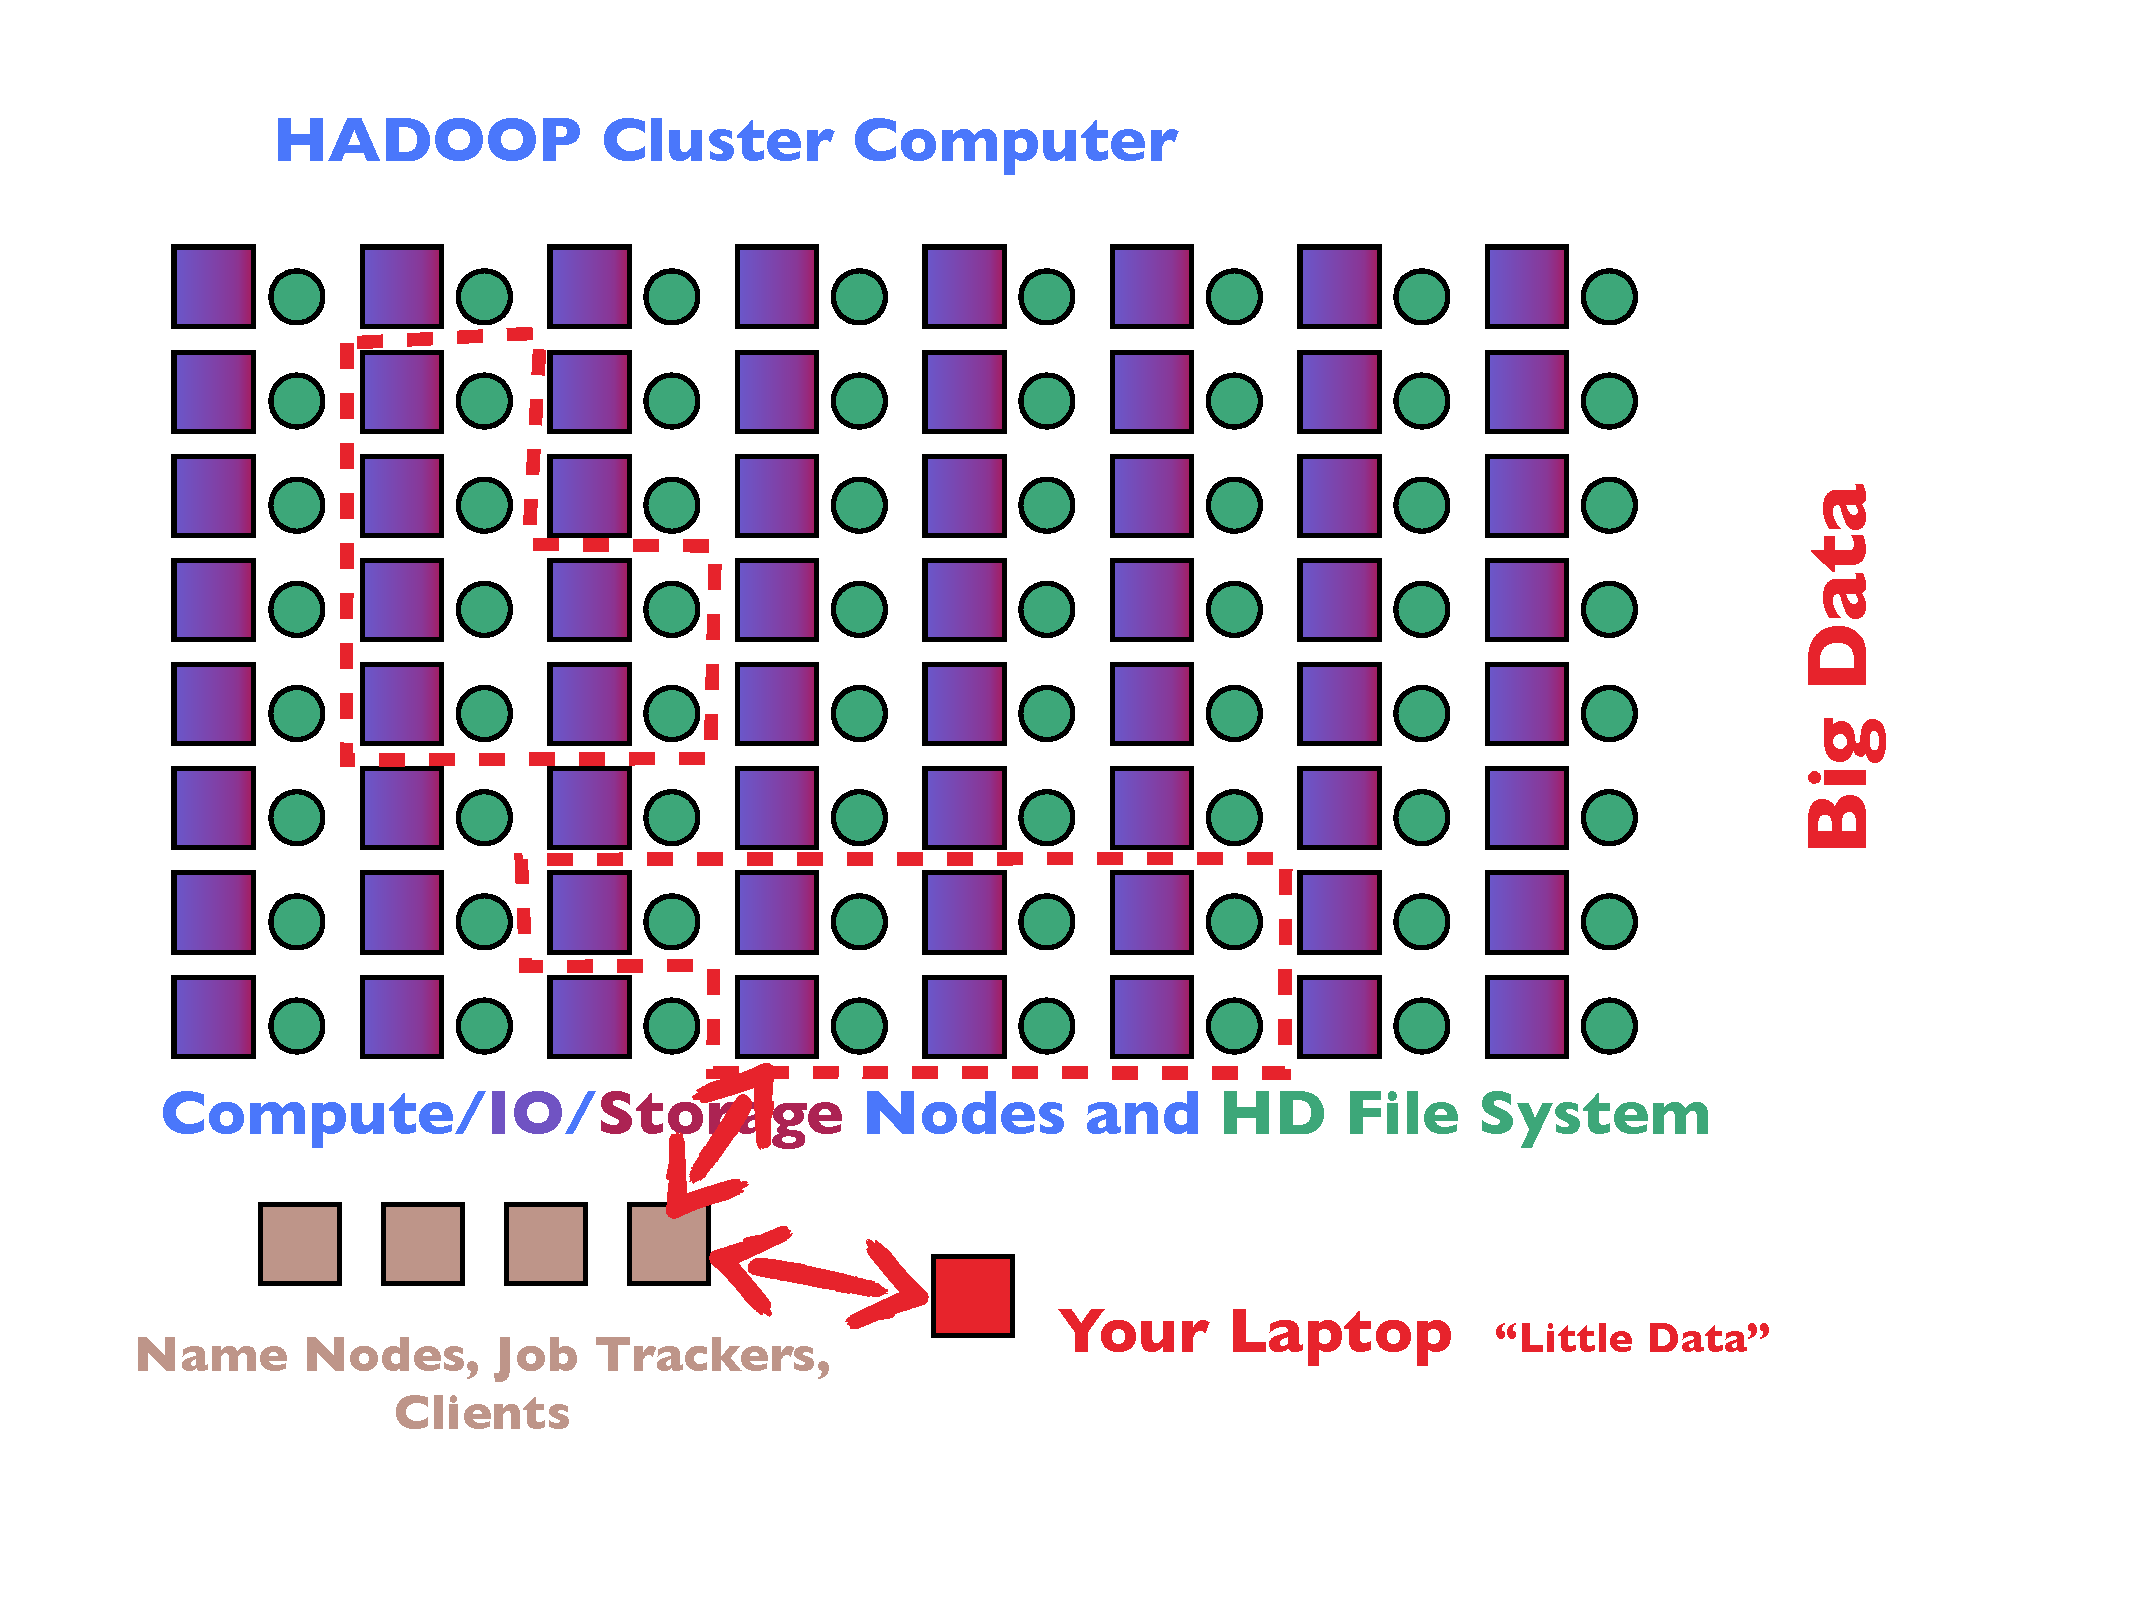
\includegraphics[trim=2cm 0cm 0cm 0cm,clip=true,height=0.8\textheight]
  {../common/pics/hardware/ParallelHardware23.pdf}
\end{minipage}
\begin{minipage}{3.7cm}\small
  \begin{block}{Software}\pause
    \scriptsize OpenMP, CUDA, OpenCL, OpenACC \\[1ex]
    Libraries: PLASMA, MAGMA, CuBLAS
  \end{block}
\end{minipage}
\end{frame}

\begin{frame}{Adding NVRAM to New HPC Systems}
\begin{minipage}{8.0cm}
\includegraphics[trim=2cm 0cm 0cm 0cm,clip=true,height=0.8\textheight]
{../common/pics/hardware/ParallelHardware24.pdf}
\end{minipage}
\begin{minipage}{3.7cm}\small
  \begin{block}{Software}\pause
    \scriptsize
    Libraries: DPLASMA, CombBLAS \\[1ex]
    HADOOP fades, Spark emerges
  \end{block}
\end{minipage}
\end{frame}

\begin{frame}{HPC Libraries: 30+ Years of Research and Development}
\includegraphics[height=\textheight]
{../common/pics/hardware/ParallelHardware25.pdf}
\end{frame}

\begin{frame}{R and \pbdR R Interfaces to HPC Libraries}
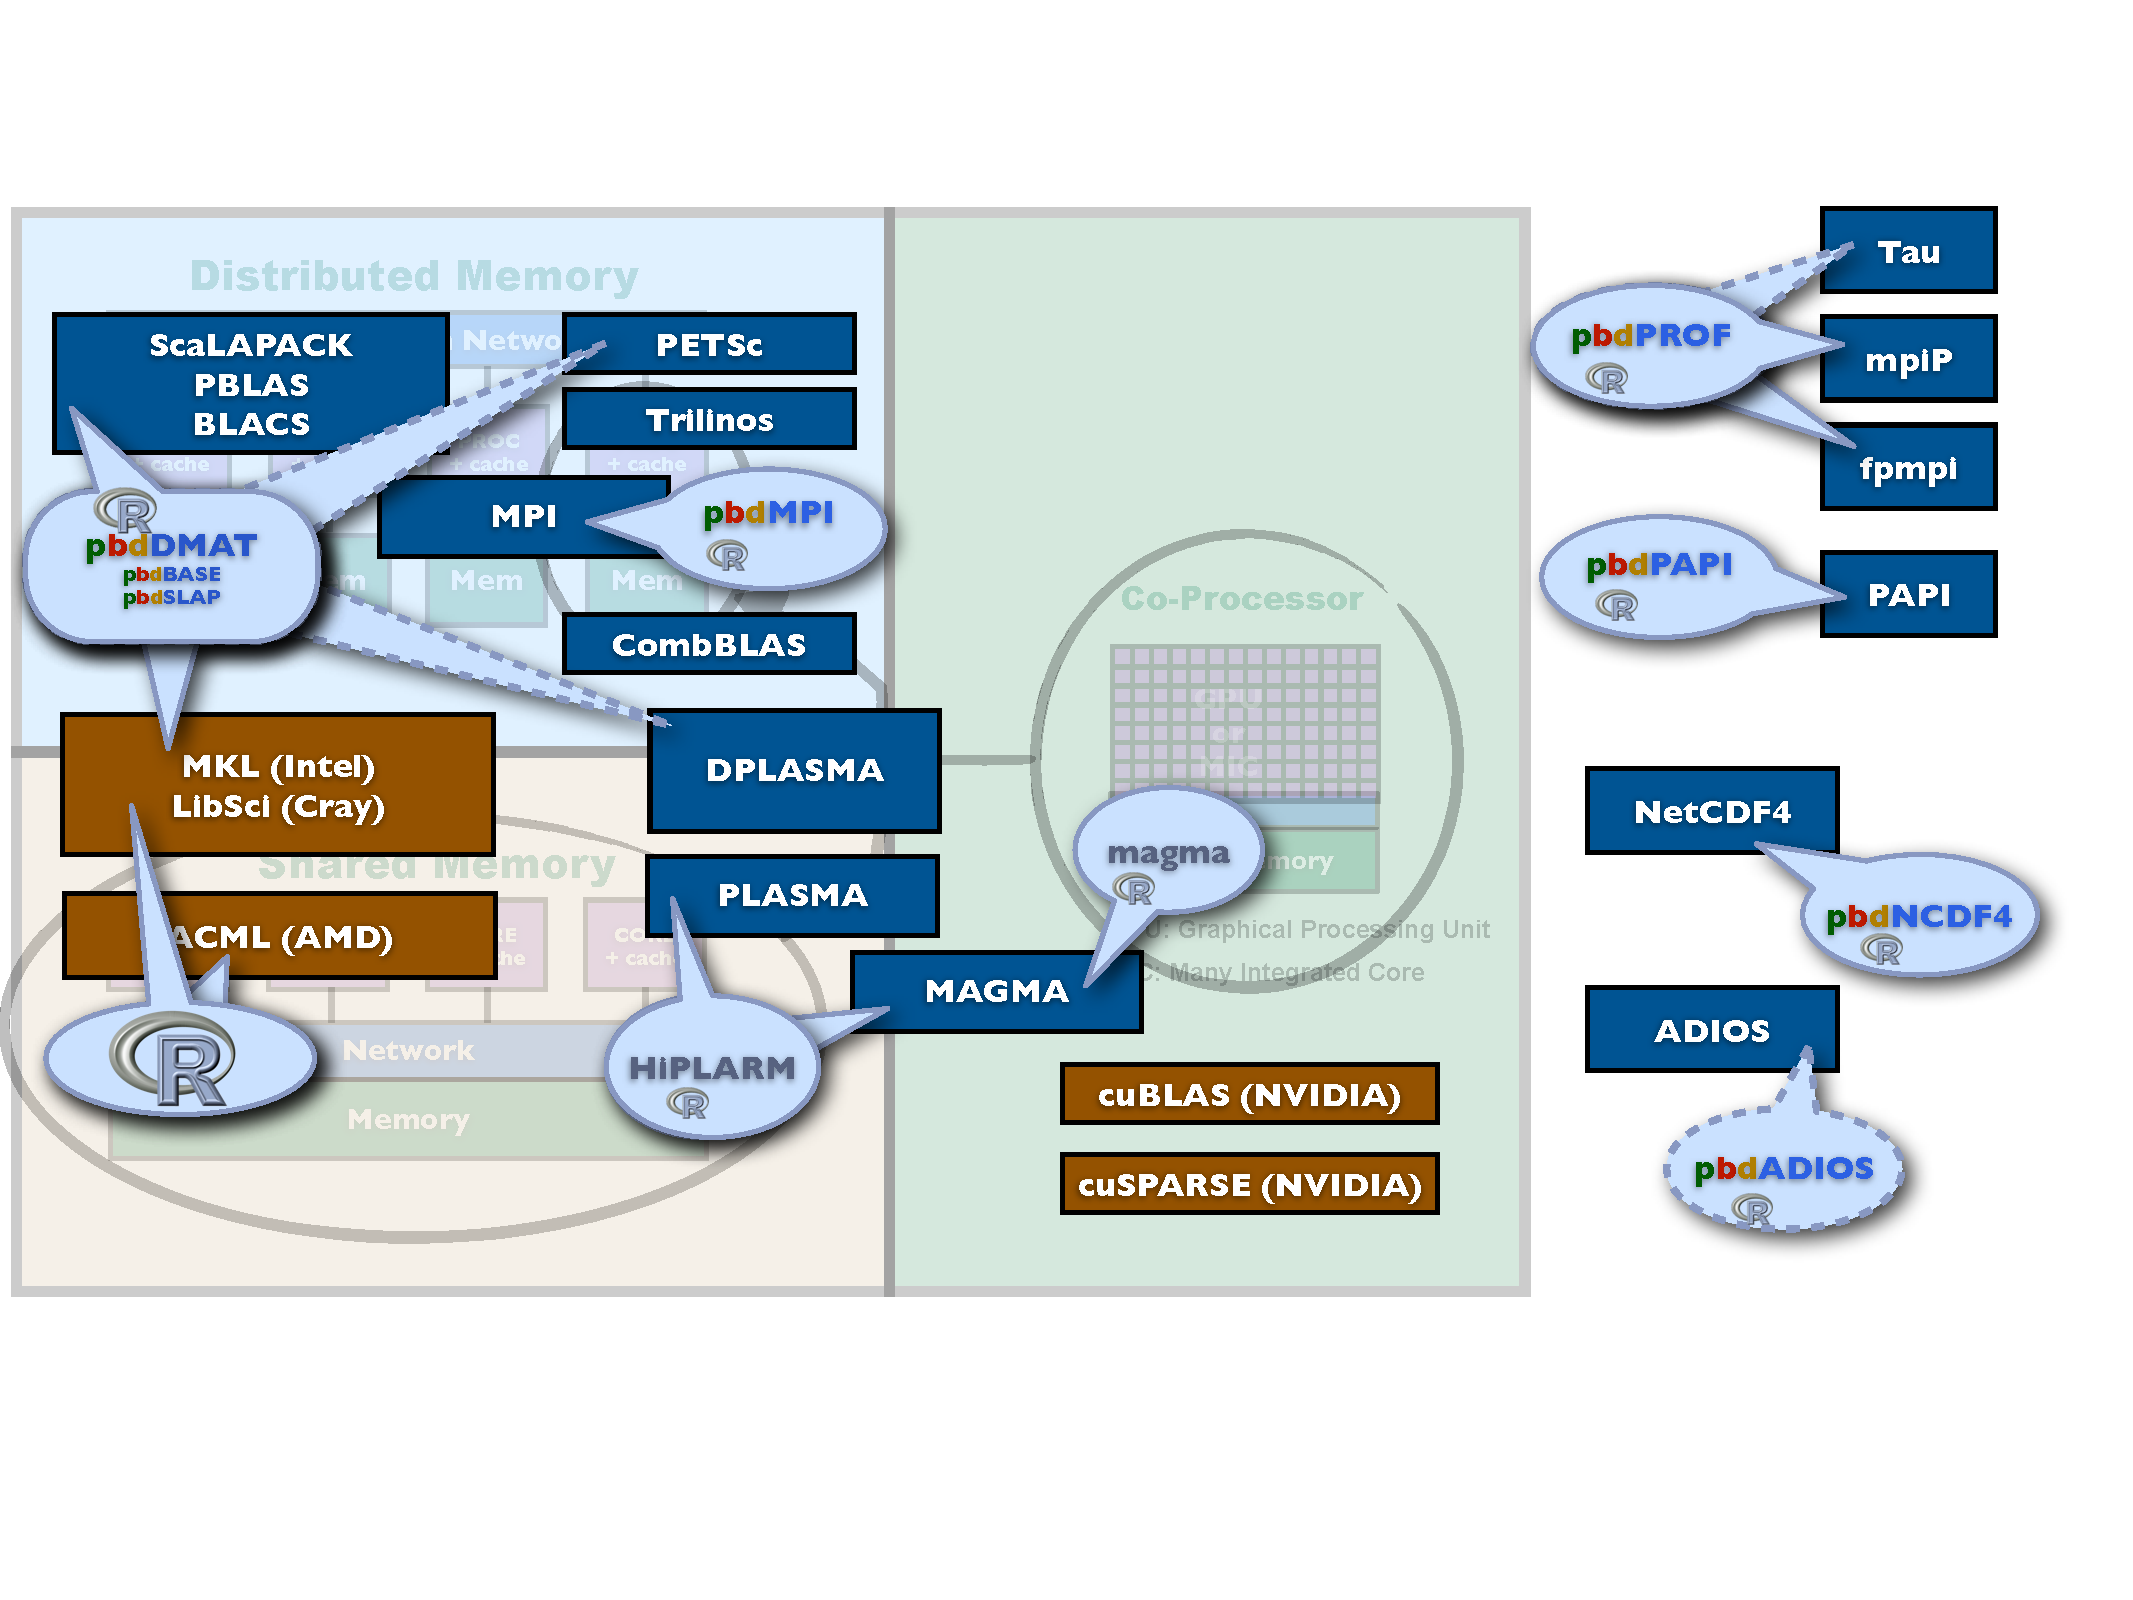
\includegraphics[height=\textheight]
{../common/pics/hardware/ParallelHardware26.pdf}
\end{frame}

% \begin{frame}{HPC Cluster File System Evolution}
%   \includegraphics[trim=2cm 0cm 0cm 4cm,clip=true,height=0.3\textheight]
%   {../common/pics/hardware/ParallelHardware23.pdf}
%   \includegraphics[trim=3cm 0cm 0cm 4cm,clip=true,height=0.3\textheight]
%   {../common/pics/hardware/ParallelHardware22.pdf}\hfill
%   \includegraphics[trim=2cm 0cm 0cm 4cm,clip=true,height=0.3\textheight]
%   {../common/pics/hardware/ParallelHardware24.pdf} \\
%   \begin{itemize}
%   \item HPC separates disk storage from compute nodes
%   \item HPC brings NVRAM to compute nodes
%   \item From Slow to Fast: Disk - Storage Server - NVRAM - Other
%     node memory - same node memory
%   \item More memory hierarchy within node
%   \end{itemize}
% \end{frame}

%\begin{frame}{\pbdR Interfaces to Libraries: Sustainable Path}
%\includegraphics[height=1.05\textheight]
%{../common/pics/hardware/ParallelHardware14.pdf}
%\end{frame}

%\begin{frame}{Low level R Interfaces to Native Tools}
%\includegraphics[width=0.95\textheight]
%{../common/pics/hardware/ParallelHardware22.pdf}
%\includegraphics[width=0.95\textheight]
%{../common/pics/hardware/ParallelHardware23.pdf}
%\end{frame}

